\emph{Konstruktion:} Man zeichnet $\vec F_2$ in einem gewählten Massstab. Um den Anfangspunkt schlägt man einen Kreisbogen mit Radius $F_\text{R}$, um die Spitze von $\vec F_2$ einen Kreisbogen mit Radius $F_1$. Der Schnittpunkt ist die Spitze von $\vec F_\text{R}$; die Seite von der Spitze von $\vec F_2$ zum Schnittpunkt ist die verschobene Kraft $\vec F_1$. Der Winkel $\alpha$ zwischen $\vec F_1$ und $\vec F_2$ lässt sich mit dem Winkelmesser ablesen.
\begin{center}
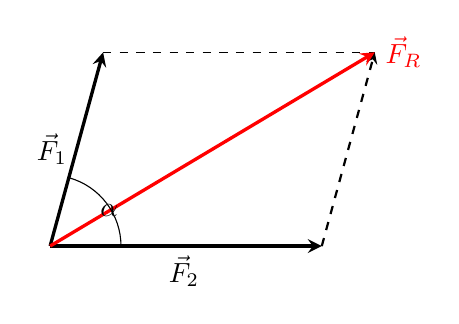
\begin{tikzpicture}[>=stealth]
 \draw[->, very thick] (0,0) -- (3.45,0);
 \node[below] at (1.7,0) {$\vec F_2$};
 \draw[->, very thick] (0,0) -- (0.673,2.46);
 \node[left] at (0.34,1.23) {$\vec F_1$};
 \draw[->, thick, dashed] (3.45,0) -- (4.123,2.46);
 \draw[dashed] (0.673,2.46) -- (4.123,2.46);
 \draw[->, very thick, red] (0,0) -- (4.123,2.46) node[right] {$\vec F_\text{R}$};
 \draw (0.9,0) arc (0:74.7:0.9);
 \node at (0.75,0.45) {$\alpha$};
\end{tikzpicture}
\end{center}

\emph{Rechnung:} Im Dreieck aus $\vec F_2$, verschobenem $\vec F_1$ und $\vec F_\text{R}$ liegt der Winkel $\SI{180}{\degree}-\alpha$ gegenüber von $F_\text{R}$. Der Kosinussatz ergibt
\begin{align}
 F_\text{R}^2 &= F_1^2+F_2^2+2\,F_1F_2\cos\alpha
\end{align}
und aufgelöst
\begin{align}
 \alpha &= \alFF \\
   &= \arccos\frac{\left(\FRk\right)^2-\left(\FEa\right)^2-\left(\FEb\right)^2}{2\cdot\FEa\cdot\FEb} \\
   &= \alF \approx \result{\alFP{0}{2}}
\end{align}
